\section{Methods}\label{sec:methods}

This retrospective study audited covariate adjustment in patient-level classification of epilepsy from first-session clinical EEG recordings in the public \textit{Temple University Hospital EEG Epilepsy Corpus} (TUEP) v2.0.1 \cite{veloso2017,obeid2016}.
The object of the audit was a three-view fusion pipeline (F2) and its components; F2 is treated as a test case, not as a validated final model.
The audit compared the pipeline with and without covariate adjustment under null experiments, against non-EEG baselines, within matched strata, and after selection over stored candidates, on identical patient-level partitions (\figref{fig:alur}).
The covariate adjustment that was originally planned fitted the correction on training controls only (V0); the leakage test showed that this choice leaked covariates, so the main evaluation used adjustment on all training patients (V4 and V5).

\input{\naskahdir/gambar_alur_audit}

\subsection{Design, data, and ethics}\label{sec:desain}

The data come from TUEP version 2.0.1, the epilepsy subset of the \textit{Temple University Hospital} (TUH) clinical EEG corpus distributed by the \textit{Neural Engineering Data Consortium} (NEDC) \cite{veloso2017,obeid2016}: 200 patients (100 with epilepsy, 100 without), each represented by the first session in the corpus (not necessarily the earliest EEG of the patient; 2003--2013). The description by Veloso et al. refers to an early version of the corpus; the figures for version 2.0.1 in this manuscript come from the local index.
TUEP contains de-identified recordings that NEDC distributes to registered users under its data use terms; this secondary analysis collected no new data and had no contact with patients. \ISI{ethics approval or exemption that applies to the authors' institution, with its basis; no number is invented}
Two public cohorts tested the transfer of predictions. Kural (Zenodo 4688758) contains 100 video-EEG subjects with a single 11--14 s segment centered on a sharp wave \cite{kural2020}; one subject (S49; peak-to-peak amplitude above 800~$\mu$V in the central window) was excluded, leaving 99. Emotiv (Zenodo 1252141) contains resting-state recordings of 313 subjects on a consumer-grade device, with eyes-closed and eyes-open periods, and was analyzed exploratorily \cite{vanhees2018}; 290 subjects had a clean eyes-closed window that was analyzed (157 with epilepsy, 133 without). The record lists 319 subjects with 14-channel recordings (its description gives 301); 313 remained after excluding two subjects without a recording file and four removed on the original investigators' notes, and only the 10 channels shared with TUEP were used. The other 23 subjects had no eyes-closed window that passed the label-free artifact thresholds (peak-to-peak amplitude and head movement, median plus three median absolute deviations per country). The TUEP model was applied to Kural without retraining. The I2 features came from one 10 s window at the center of the segment, age and sex from the Kural file, and the era column was zero (reference era 2012). For Emotiv, a band-power model trained on TUEP was applied in two settings: with frozen TUEP preprocessing statistics, and after standardizing each cohort with its own feature means and SDs; the second setting uses the unlabeled features of all 290 target subjects (transductive, without labels) and is an unsupervised adaptation, not a frozen deployment.

\subsection{Participants, EEG acquisition, and reference standard}\label{sec:partisipan}

All 200 patients were included and only the first session was analyzed (one prediction per patient; later sessions were used only for two descriptive stability analyses).
Of 265 first-session recordings, 3 were excluded because they were too short and 13 because they had no clean window, so 249 recordings (78.3 hours) were analyzed without excluding any patient.
The EDF recordings used 19 electrodes in the 10--20 system (250 Hz in 190 patients, 256 Hz in 9, 400 Hz in 1; average-reference montage in 149 patients and linked ears in 51). Age and sex were available for all patients. The device was read from the recording field of the EDF header; masked entries were counted as ``other'', and for the year $\times$ device strata all devices except X and Intuition formed one group.
The labels came from TUEP curation based on the session report, clinical history, medication taken at the time of recording, and epilepsy-related EEG features (keywords reviewed manually) \cite{veloso2017}. The estimand is therefore discrimination of the TUEP label, not of an independent clinical diagnosis; the label is not fully independent of the signal. Inter-rater agreement and epilepsy type are not available, and this study did not use medication data.

\subsection{Preprocessing and segmentation}\label{sec:praproses}

The signals (\figref{fig:kanal}; example window in \figref{fig:sinyal}) were trimmed of leading and trailing calibration segments, re-referenced to the average of the non-flat channels (standard deviation $\geq 0.5~\mu$V; no first-session recording had a flat channel), resampled to 200 Hz, and filtered with a zero-phase FIR filter at 0.5--45 Hz.
Recordings longer than 2 hours were treated as long-term monitoring and only their first 60 minutes were used (one first-session recording, 201 minutes); recordings up to 2 hours were used in full (the longest other first-session recording lasted 66 minutes).
Non-overlapping 10 s windows (the first and last 10 s skipped) with a channel peak-to-peak difference above 800~$\mu$V were rejected (628 of 27,596; 2.3\%; labels were not used), which yielded 26,968 clean windows (12--411 per patient; median 123). The temporal view used 4 s segments (at most 600 per patient), and the reproduced published methods used their own segmentation (S3.5).
The window length and the 800~$\mu$V threshold were set in advance and their sensitivity was not tested. All of these steps are label-free and run per recording; every step that estimates statistics across patients was fitted inside the folds (Subsection~\ref{sec:validasi}).

\begin{figure}[t]
\centering
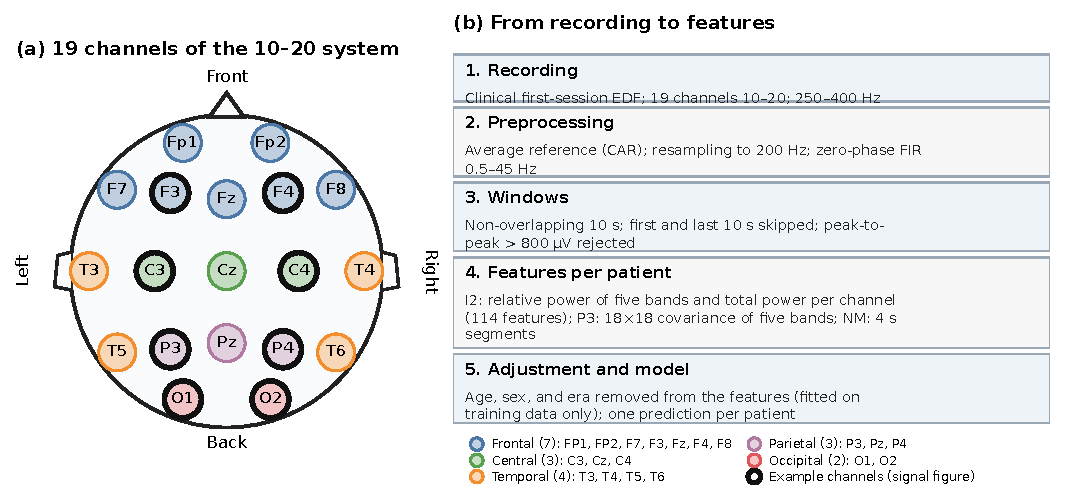
\includegraphics[width=0.88\textwidth]{figures_en/gambar_kanal.pdf}
\caption{Channels and the preprocessing workflow. (a) The nineteen electrodes of the 10--20 system are grouped into five regions (the basis of the anatomical compression analysis); thick circles mark the eight channels shown in \figref{fig:sinyal}. (b) From the first-session clinical recording to the per-patient prediction: average reference, resampling to 200 Hz, 0.5--45 Hz filter, clean 10 s windows, three feature views (I2, P3, NM), then covariate adjustment and one prediction per patient.}\label{fig:kanal}
\end{figure}

\begin{figure}[t]
\centering
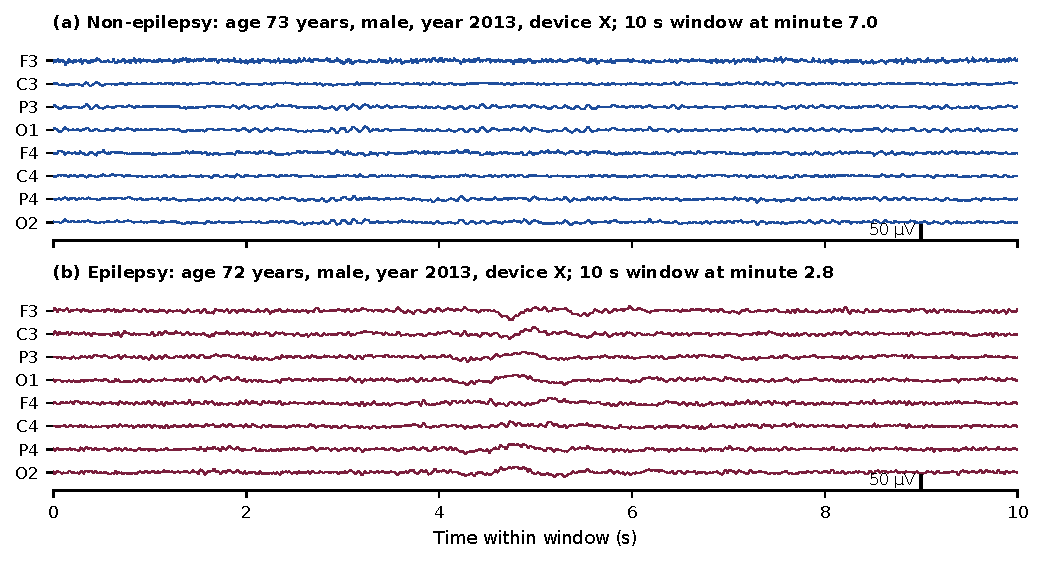
\includegraphics[width=0.85\textwidth]{figures_en/gambar_sinyal.pdf}
\caption{Example 10 s windows from the first session of a pair of patients matched on recording year (2013), device (X), sex (male), and age (72 and 73 years): (a) non-epilepsy and (b) epilepsy; eight of the 19 channels, same amplitude scale. The pair was chosen at random (seed 20261024) from 51 eligible pairs, and the window whose \textit{line length} was closest to the median of the recording was chosen, not the one that looked most abnormal. No part is marked as a seizure: TUEP v2.0.1 contains only EDF files without seizure annotations or clinical reports, both windows come from routine interictal EEG, and this study classifies patients and does not detect seizures. The visible differences cannot be interpreted as a marker of epilepsy without clinical reading.}\label{fig:sinyal}
\end{figure}

\subsection{Audit design: null experiments and decision rules}\label{sec:sensitivitas}

The leakage test followed Hamdan et al. \cite{hamdan2023}: the EEG features were permuted between patients before the split while each patient kept its label and covariates, and the complete pipeline was run with and without adjustment on the same folds (\tabref{tab:definisi_null}; pseudocode in S1.1). Under H1 the EEG carries no information about the label or the covariates, but the label--covariate association is preserved; an AUC above chance after adjustment then indicates adjustment-induced leakage. H2a and H2b keep the association of the EEG with era or with year and device. Rounds 28--29 permuted each patient-level feature separately, and later rounds moved the whole EEG block of a patient (all windows and features together), so that within-patient structure was kept.

\input{\naskahdir/tabel_definisi_null}

Rule R1 (absolute): a mean AUC on uninformative features $\leq 52.0$ together with a mean $+\,1.645\,\mathrm{SE}$ $\leq 54.0$ meant no evidence of leakage, a mean AUC above 55 meant leakage, and anything else was uncertain.
Rule R2 (paired, H1 only): the difference from the unadjusted control on identical folds and permutations $\leq 1.0$ pp and a one-sided 95\% upper bound $\leq 3.0$ pp meant no evidence, a difference above 3.0 pp meant leakage, and anything else was uncertain; for H2a, a legitimate era effect remains, so only R1 applies.
The SE in both rules is the Monte Carlo error over replicates on the same 200 patients; it does not include the variation expected in new patients.
Rounds 28, 29, and 36--38 computed the rules on the pooled AUC; R1 was applied retrospectively in rounds 28 and 29, with the original thresholds of 52 and 55 in round 29 (\tabref{tab:kebocoran_badan}). Rounds 40 and 46 computed them on the per-fold AUC with the same thresholds.
V1--V3 were tested on I2, V4 on I2 and NM (reduced null test), and V5 on P3.
The properties of the rules were estimated in round 49 (follow-up analysis; plan hashed before computation) from stored replicates: decision frequencies when leakage is absent (unadjusted pipelines and simulation cells without a label--covariate association) and when leakage of known size is present (V0 and simulation cells whose long-run mean exceeds the leakage threshold), for 10 to 100 replicates, with Monte Carlo 95\% CIs; parametric operating curves; the number of published decisions that change under stricter or looser thresholds fixed in advance; and the patient-sampling SD of the mean null AUC compared with its Monte Carlo SE (100 replicates of C1 and V4 rerun with stored predictions). The rules and their thresholds were fixed before this analysis (R1 in rounds 29--30, R2 in rounds 37--38) and were not changed in it; the analysis evaluates the rules without recalibrating them.
The confounder tests followed Spis\'ak \cite{spisak2022} with our own implementation: the partial test asks whether out-of-fold scores depend on a confounder given the label ($H_0$: score $\perp$ confounder $\mid$ label; confounder permuted within each label class), and the full test asks whether scores depend on the label given the confounder ($H_0$: score $\perp$ label $\mid$ confounder; label permuted within confounder cells), with 10,000 permutations each; \texttt{mlconfound} 0.21.3 was used only for verification. Not rejecting the partial null does not show that confounding is absent, and rejecting the full null does not show a pure disease signal.

\subsection{Models under audit}\label{sec:model}

F2 is the arithmetic mean of the probabilities of three views, with no learned parameters.
Covariate adjustment fitted a linear regression of the features on [1, age, sex, era indicator] by ordinary least squares on all training patients without labels, and divided the residuals by the training residual standard deviation to obtain the features (\eqref{eq:norm}).
\begin{equation}\label{eq:norm}
\hat{\mathbf{B}}=\arg\min_{\mathbf{B}}\sum_{q\in\mathcal{P}_{\mathrm{tr}}}\left\|\mathbf{x}_q-\mathbf{B}^{\top}\mathbf{d}_q\right\|^{2},\qquad
\mathbf{z}_p=\left(\mathbf{x}_p-\hat{\mathbf{B}}^{\top}\mathbf{d}_p\right)\oslash\hat{\mathbf{s}}
\end{equation}
The originally planned adjustment (V0) fitted the coefficients only on training non-epilepsy patients and leaked covariates: the residuals of the training controls were orthogonal to the design, whereas those of the patients with epilepsy were not. Adjustment on all training patients (V4; V5 for P3) was therefore used. This approach was inspired by normative modeling \cite{rutherford2022,rutherford2023} without using the controls as a reference.
The spectral view (I2) used the log relative power of five bands (delta, theta, alpha, beta, gamma; 1--45 Hz) and the log total power on 19 channels from the Welch spectrum (114 features), the median over windows per patient, plus age and sex. The classifier was L2 logistic regression with balanced class weights and $C$ from nine values $10^{-3}$--$10^{1}$ chosen by inner 5-fold cross-validation scored by AUC. The events-per-predictor ratio was only 0.86.
The spatial view (P3) used the $18\times18$ covariance of five bands after projection orthogonal to the average-reference direction (shrinkage $10^{-3}\,\mathrm{tr}(\mathbf{C})/18$). The covariances were aligned to a single global reference, namely the arithmetic mean of the training-window covariances \cite{zanini2018,he2020}, then mapped to the tangent space (855 features) and averaged per patient. The next steps were PCA with 50 components, adjustment on the components, addition of age and sex, and the same L2 logistic regression.
The temporal view (NM, NormMamba) used a sequence of adjusted 4 s segments, two Mamba layers \cite{gu2023}, bidirectional \cite{wang2025eegmamba}, attention pooling, and a patient-summary branch (median token, age, sex; 155,586 parameters at $d=64$); training and configuration selection are described in S1.2. I2, P3, and NM all receive age and sex after adjustment, so their outputs combine EEG and non-EEG information. The composition of F2 was chosen after the AUCs of its components were known, so selection optimism cannot be ruled out.

\subsection{Validation design, estimands, comparators, and statistics}\label{sec:validasi}

The evaluation used repeated patient-level cross-validation: 10 repetitions of five stratified folds (160 train, 40 test), that is, the same 50 canonical splits for all models. The split was made first and all fitting was done on the training data of that fold \cite{varma2006,rosenblatt2024,delpup2025,brookshire2024}.
In the main pipeline the label-free transforms (scaling, adjustment, reference covariance, PCA) were fitted on the whole outer training fold before the inner selection of $C$, and the NM adjustment included the validation patients used for early stopping; outer test patients were never used (S1.2), but the inner validation patients contributed label-free statistics to the transforms. As a sensitivity analysis (round 49; ``strict nesting''), every transform was refitted inside each inner training split, and the NM adjustment was fitted without the validation patients.
The automated leakage checks passed on all 50 folds (perturbation of test data and labels; 300 checks) for I2 with V4, P3 with V5, and NM with V4, plus residual orthogonality and a global label permutation.
Design choices were iterated over 44 rounds and six follow-up rounds (45--50) on the same patients and folds without a hidden test set. Each round was planned in a version-controlled document (committed to Git in rounds 3--27, hashed with SHA-256 in rounds 28--50) written after the results of earlier rounds were known; these are follow-up, not confirmatory, analyses (S1.5).
The comparators were C1 (without covariate adjustment), an acquisition-metadata baseline without EEG, a demographic baseline, and three published methods reproduced per patient (Tang-F, Rohira-F, DNM-F) \cite{rohira2023,tang2024,myers2025}. The metadata baseline used nested L2 logistic regression like I2 on the original sampling frequency, the number of signals, the logarithm of the total duration of the first session, the numeric recording year, and the binary-coded montage and device. To measure EEG information beyond all non-EEG predictors (round 49), N0 combined the metadata with age and sex, N1 added the 114 adjusted I2 features, and N2 added the 114 unadjusted band powers, all with strict nesting. The \textit{pretrained} models comprised frozen BENDR, LaBraM, and CBraMod embeddings with logistic regression, as well as LaBraM and CBraMod fine-tuned with the official recipes \cite{kostas2021,jiang2024,wang2025cbramod}. The equal-treatment analysis was run after the main results were known and is therefore exploratory.
The primary metric was the per-fold AUC (mean of 50 folds) with a Nadeau--Bengio corrected 95\% CI \cite{nadeau2003}, $t=\bar{d}/\sqrt{(1/J+n_{2}/n_{1})\,s_{d}^{2}}$ ($J=50$, $n_{1}=160$, $n_{2}=40$); this correction addresses the dependence between cross-validation folds but does not capture the uncertainty of the development process. The pooled AUC (patient \textit{bootstrap} CI) was secondary, and the within-strata analyses used the AUC of scores averaged over the 10 repetitions, which gives higher values (S1.3). The AUC is reported in percent and differences in percentage points (pp); values were rounded half up. The study size was not determined a priori because all of TUEP was used. At a pooled AUC of 69.4, the Hanley--McNeil 95\% CI half-width is $\pm 7.3$ pp and 422 patients would be needed for $\pm 5.0$ pp. The smallest detectable difference at 80\% power (corrected $t$-test; post hoc) is 7.7 pp for F2 versus I2, 8.9 for F2 versus C1, 7.0 for I2 versus C1, and 15.9 for F2 versus the metadata baseline.
As a sensitivity analysis, the main differences were also computed with a patient-level bootstrap (2,000 replicates; test-sample variation only; S2). Differences were tested with the corrected $t$-test; Holm \cite{holm1979} was used within each test family and Benjamini--Hochberg \cite{bh1995} for FDR as an approximation (the tests share patients and folds). Holm within a round does not control the error across rounds; the questions, endpoints, families, and corrections are listed in S1.4. A post hoc analysis (plan hashed as 1427aee528a6, created before computation) tested equivalence of 12 pairs with TOST at a margin of 3 pp and, as sensitivity analyses, 2 and 5 pp, a convention without clinical basis (Nadeau--Bengio variance; Holm per margin). The pairs were the four F2 variants, I2, and C1 against metadata or C1, and F2 against I2.
The family F2 versus LaBraM-FT and CBraMod-FT was defined in round 30; the registry of 89 tests under V0 (rounds 3--26) was superseded because V0 leaked and is kept in the repository as an analysis trail.
The within-strata analysis compared only epilepsy--non-epilepsy pairs from the same year $\times$ device stratum, with an age caliper $k\in\{5,10,15\}$ years; every pair had equal weight, and the CI came from a bootstrap that resampled patients within each stratum and rebuilt the pairs (2,000 replicates), because pairs that share a patient are not independent. Round 49 reported the patients behind the pairs and two weightings (equal weight per stratum; largest stratum removed).

\subsection{Simulation, plasmode, within-patient structure, and selection correction}\label{sec:metode_peta}

\begingroup\emergencystretch=\dimexpr\baselineskip+\baselineskip+\baselineskip\relax
Unmet predictions and deviations in rounds 39--50 are reported in Supplementary Material S2.
The simulation (round 39) generated clustered data without a disease signal (base cell: 200 patients, 50 windows per patient, 50 features; varied one factor at a time to 100 or 500 patients, 10 or 200 windows, 10 or 200 features, or unequal window counts of 12--200 per patient, $50e^{0.6z}$ rounded and truncated; 20 to 100 replicates per cell; normal, lognormal, $t$, chi-squared, or artifact-contaminated distributions) with covariates mimicking TUEP and a label--covariate association strength $s\in\{0,0.5,1\}$. The simulation compared transformations (raw, symlog, rank-normal with training-data quantiles, log), adjustments (none, per window, per patient), and classifiers (logistic regression, \textit{random forest}, XGBoost, MLP, Bi-LSTM) on the same data and folds.
Round 40 recomputed R1 and R2 on the per-fold AUC and tested two exploratory hypotheses (H40-1 and H40-3; Subsection~\ref{sec:peta}).
To isolate the within-patient structure (round 49), the simulation held the number of patients (200), the marginal feature distribution (normal, lognormal, or 1\% contamination), and the covariates fixed, and varied the latent intraclass correlation (ICC) of the windows (0, 0.3, 0.7, 0.95), the number of windows per patient (10, 50, 200), and the order of aggregation: adjustment per window with a window-level \textit{random forest} (A), adjustment from patient means applied to windows (B), and aggregation to patient means before adjustment with a patient-level \textit{random forest} (C), each paired with the same classifier without adjustment, plus patient-level logistic regression. The latent ICC refers to the normal variable before the marginal transformation; the observed ICC of the lognormal features was 0.20, 0.59, and 0.92 at the three nonzero values, and at most 0.04 with 1\% contamination. There were 20 replicates per cell, fixed in advance from a target SE of 0.6 pp (not reached for the tree arms; S2.15). The primary family (Holm, two tests; lognormal, 50 windows) was the change in leakage of A from latent ICC 0 to 0.95 (D1) and the difference between A and C at ICC 0 (D2).
The plasmode (round 42) used real EEG features (I2; the Rohira window with 48 features; Tang per-second features; NM segments) and synthetic labels. Labels were assigned to the 100 patients with the highest score $\gamma\eta_i+\epsilon_i$, where $\eta_i$ is the predictor of a logistic regression of the real label on the covariates, $\epsilon_i$ is standard logistic, and $\gamma\in\{0,0.5,1\}$ ($\gamma=1$ mimics the real association: covariate AUC 70.7 versus 71.0). Features were swapped between patients (H1) or within era (H2a), with 30 replicates (logistic regression, \textit{random forest}) or 20 (XGBoost, Bi-LSTM, NM). The primary family (Holm, three tests) was the AUC difference between the raw and rank-normal pipelines for the \textit{random forest}, XGBoost, and Tang. Its control: at $\gamma=0$, at least 95\% of cells had the decision ``no evidence''.
In the simulations and the plasmode, each replicate used one new stratified 5-fold patient-level split instead of the 50 canonical splits, because the data or the synthetic labels differ between replicates. Round 50 (after review; plan hashed before computation, \texttt{6e4e37e4920c}) extended the plasmode replicates of the raw tree pipelines to 120 per cell (H1, $\gamma\in\{0,1\}$; unchanged code and seeds, which reproduced the stored replicate 0 exactly) and repeated the plasmode on the independent Emotiv cohort: 299 subjects with at least five clean 10 s windows (5--27 per subject; 163 with epilepsy), raw power in the six Rohira bands on the 10 shared channels (60 features) for window-level \textit{random forest} and XGBoost, and subject-level median log band powers for logistic regression. There, synthetic labels came from the acquisition covariates recorded in that cohort (country, eyes condition recorded first, recording day, and time of day; covariate AUC for the real label 68.5), and the primary family (Holm, two tests) was the difference with minus without raw adjustment at $\gamma=1$ for the \textit{random forest} and XGBoost.
Round 43 equalized the foundation-model pipeline (embeddings averaged per patient, PCA 50, rank-normal, V4, age and sex, L2 logistic regression with six values of $C$; all refitted in each inner fold). That round also tested a 50-feature anatomical compression (relative power of five bands in five regions). The selection-optimism analysis used a stratified patient \textit{bootstrap} (2,000 replicates) of the out-of-fold predictions of the 15 main candidates or the 50 stored candidates, plus a \textit{studentized max-T} multiple-comparison test against the metadata baseline and C1 (algorithm in S1.3). It is a sensitivity analysis of selection conditional on the stored candidates; it does not repeat the adaptive process that produced them and is not an independent validation.
Round 44 removed age and sex from the final classifier (F2-Clean; the main variant, with rank-normal before V4 on a design extended by a squared age term, was set before it was run). The label ``Clean'' names the design (no age or sex input), not an absence of leakage. F2-Clean met the age rule if the partial $r^2$ of age was $<0.02$ and $p>0.10$; this rule shows that the score depends little on age linearly, not that all dependence on age is gone. The primary family (Holm, four tests) was the difference from F2, C1, and the metadata baseline, plus the 10-year caliper AUC against 50. IPW weighted the training patients by $1/P(y\mid\text{covariates})$ without changing the features, and the 30-window sensitivity analysis took at most 30 windows per patient.\par\endgroup

Codes used in the text are defined in the glossary (S1.6). In brief, F2 is the probability average of I2 (spectral), P3 (spatial), and NM (temporal), and C1 is the spectral model without covariate adjustment; V0 fits the adjustment from training controls only and V4 from all training patients (V5 is the counterpart of V4 for P3); F2-Clean is F2 without age and sex in the final classifier.

\subsection{Implementation and availability}\label{sec:implementasi}

The experiments were run on an Intel Core Ultra 9 285K processor, 62 GB of RAM, and an NVIDIA RTX 4080 SUPER 16 GB GPU (Python 3.12.3, PyTorch 2.11.0, scikit-learn 1.9.1, NumPy 2.5.2, SciPy 1.18.1, MNE 1.13.2, pyriemann 0.12). Inference per patient required 0.1 ms for I2 and 35 ms for NM, and the models were run offline without a connection to a medical record system.
The TUEP data cannot be redistributed. The code, environment, fold assignments, seeds, analysis plans with addenda, and table scripts are listed in S1.7 \ISI{repository link and licence}; reporting followed the relevant items of TRIPOD+AI \cite{collins2024tripod}.
